\section{Experimentación Y Resultados}

  Los algoritmos previamente detallados tienen muchos puntos a testear. Veamos cada uno de estos en forma detallada y con los resultados intentemos responder a la pregunta original: ¿qué estrategia debo tomar para posicionar mi sitio en internet?

  \begin{itemize}
    \item{Convergencia de Page Rank}
    \item{Convergencia de Hits}
    \item{Comparación de tiempos}
    \item{Comparación de calidad}
    \item{Comportamiento}
  \end{itemize}


\subsection{Casos de prueba}
   A continuación se listarán los casos utilizados en las experimentaciones para mayor comprensión de los casos.

	\begin{itemize}
		\item MOVIES: Este caso incluye 5797 páginas
		\item ABORTION: Este caso incluye 2293 páginas
		\item GENETIC: Este caso incluye 3468 páginas
		\item STANFORD: Este caso incluye 281903 páginas
		\item GOOGLE: Este caso incluye 916428 páginas
	\end{itemize}  

\subsection{Convergencia de Page Rank} 

La convergencia de dicho algoritmo ocurrirá cuando la norma Manhattan de los vectores de la iteración anterior y la del actual sea cero(o a un valor relativamente cerca, esta cercanía estará dada por una tolerancia que para los casos presentados son cero). Es ahí cuando tendremos la respuesta final.\\
Para evaluar el comportamiento de la norma manhattan variaremos la probabilidad del navegante aleatorio, el cual de ahora en más lo denotaremos como el parámetro \textbf{c}.\\
A continuación se muestran los resultados para cuatro tests de como evoluciona la norma a lo largo de las iteraciones y como varía la misma con distintos c, y que luego discutiremos más adelante.
Cabe aclarar que expresamos los valores de la norma en escala logarítmica para una mejor visualización y para que se obtenga un mejor entendimiento de como disminuye de a varias magnitudes en cada iteración.


% \begin{figure}
% \begin{center}
       % 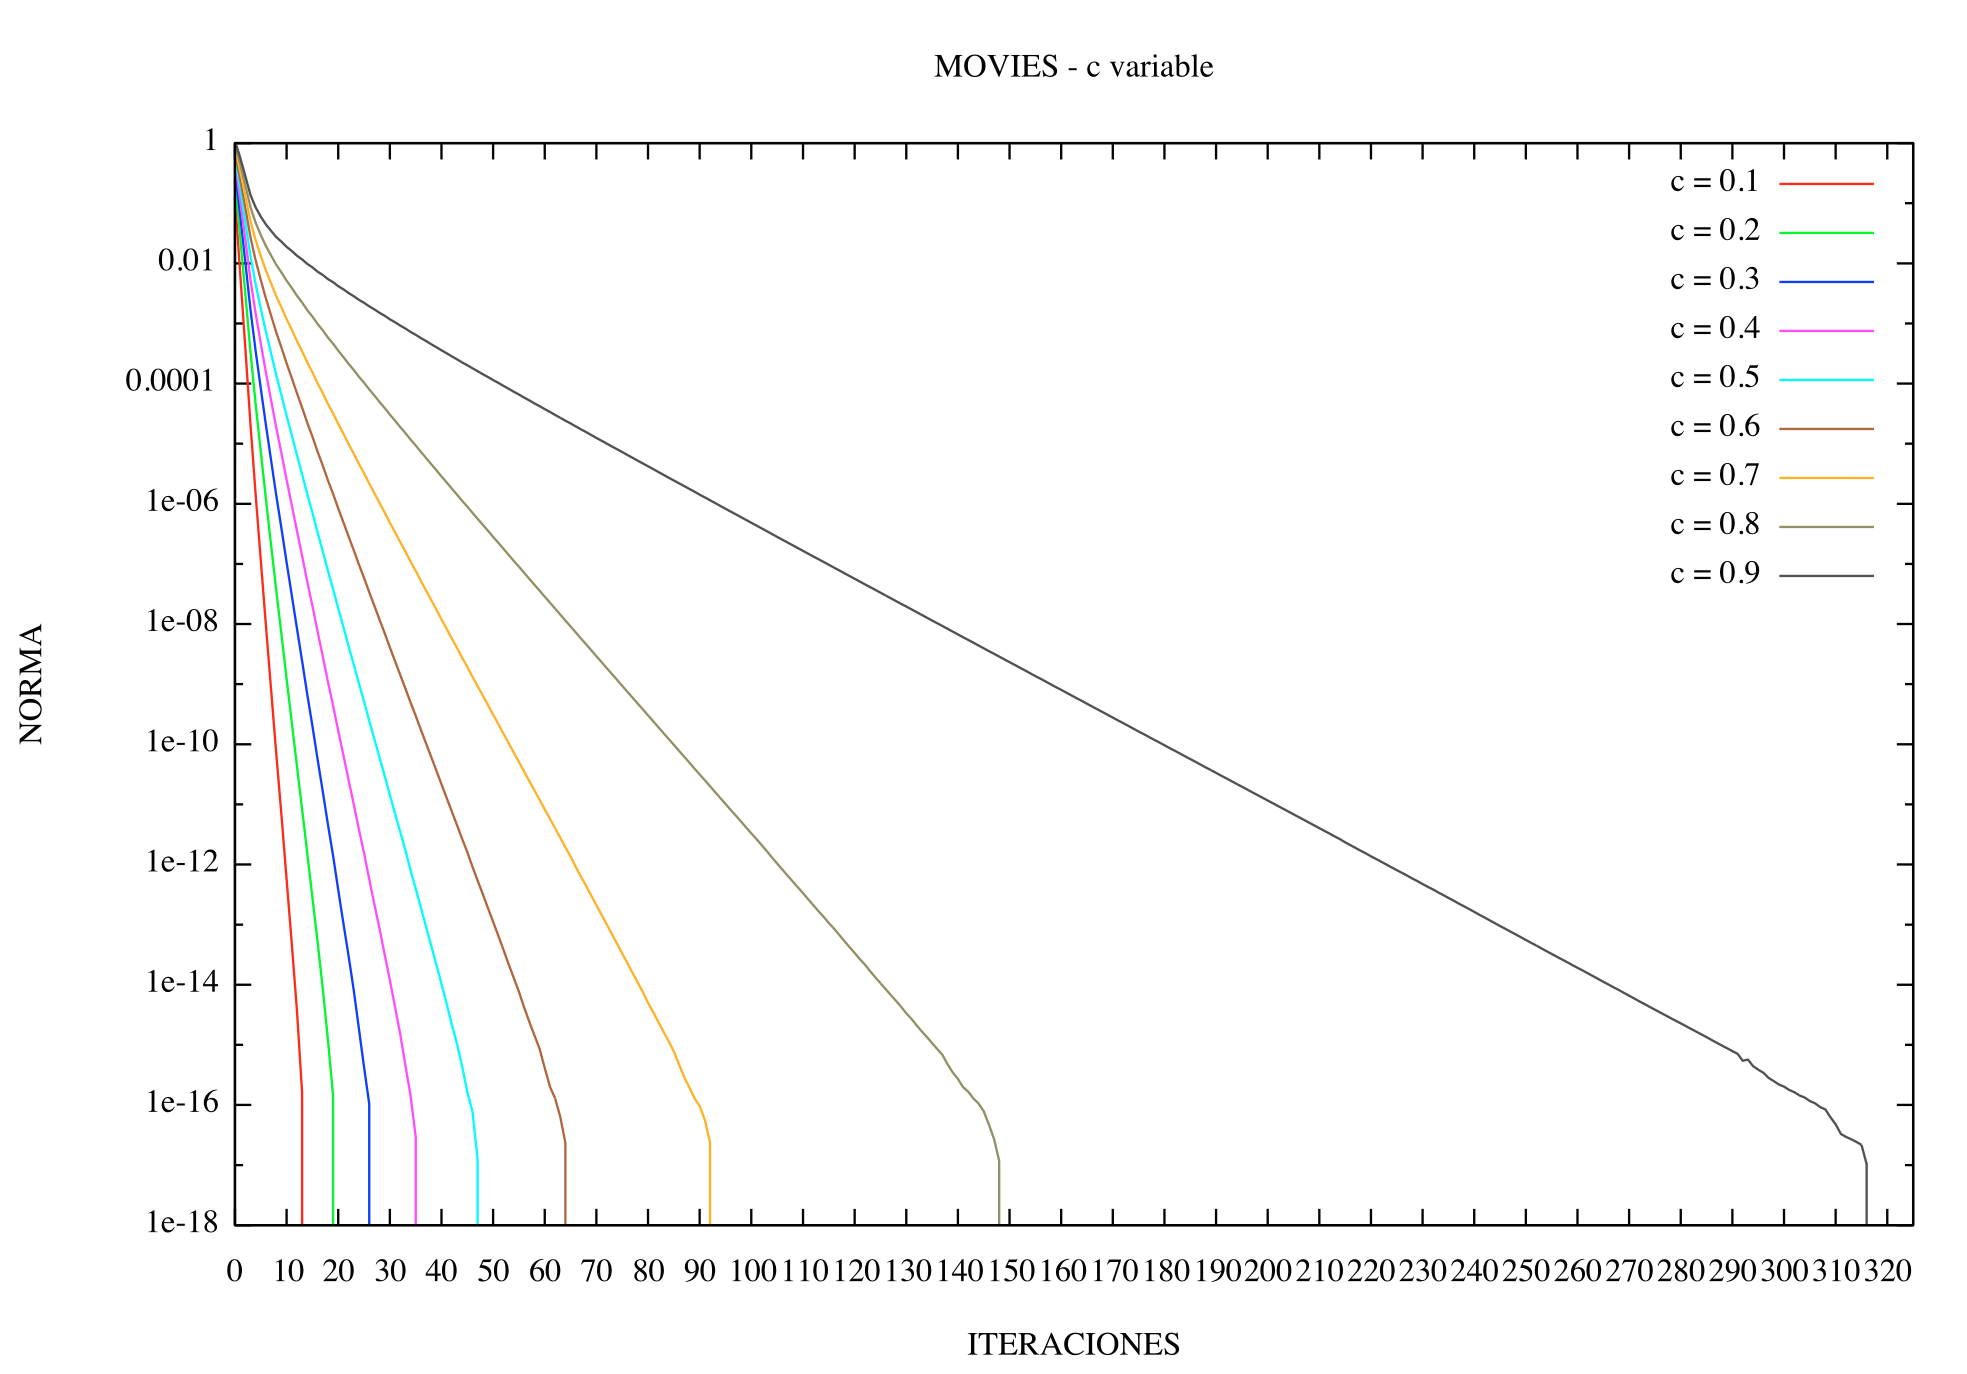
\includegraphics[scale=0.5]{imagenes/pagerank_movies_norma.png}
        % 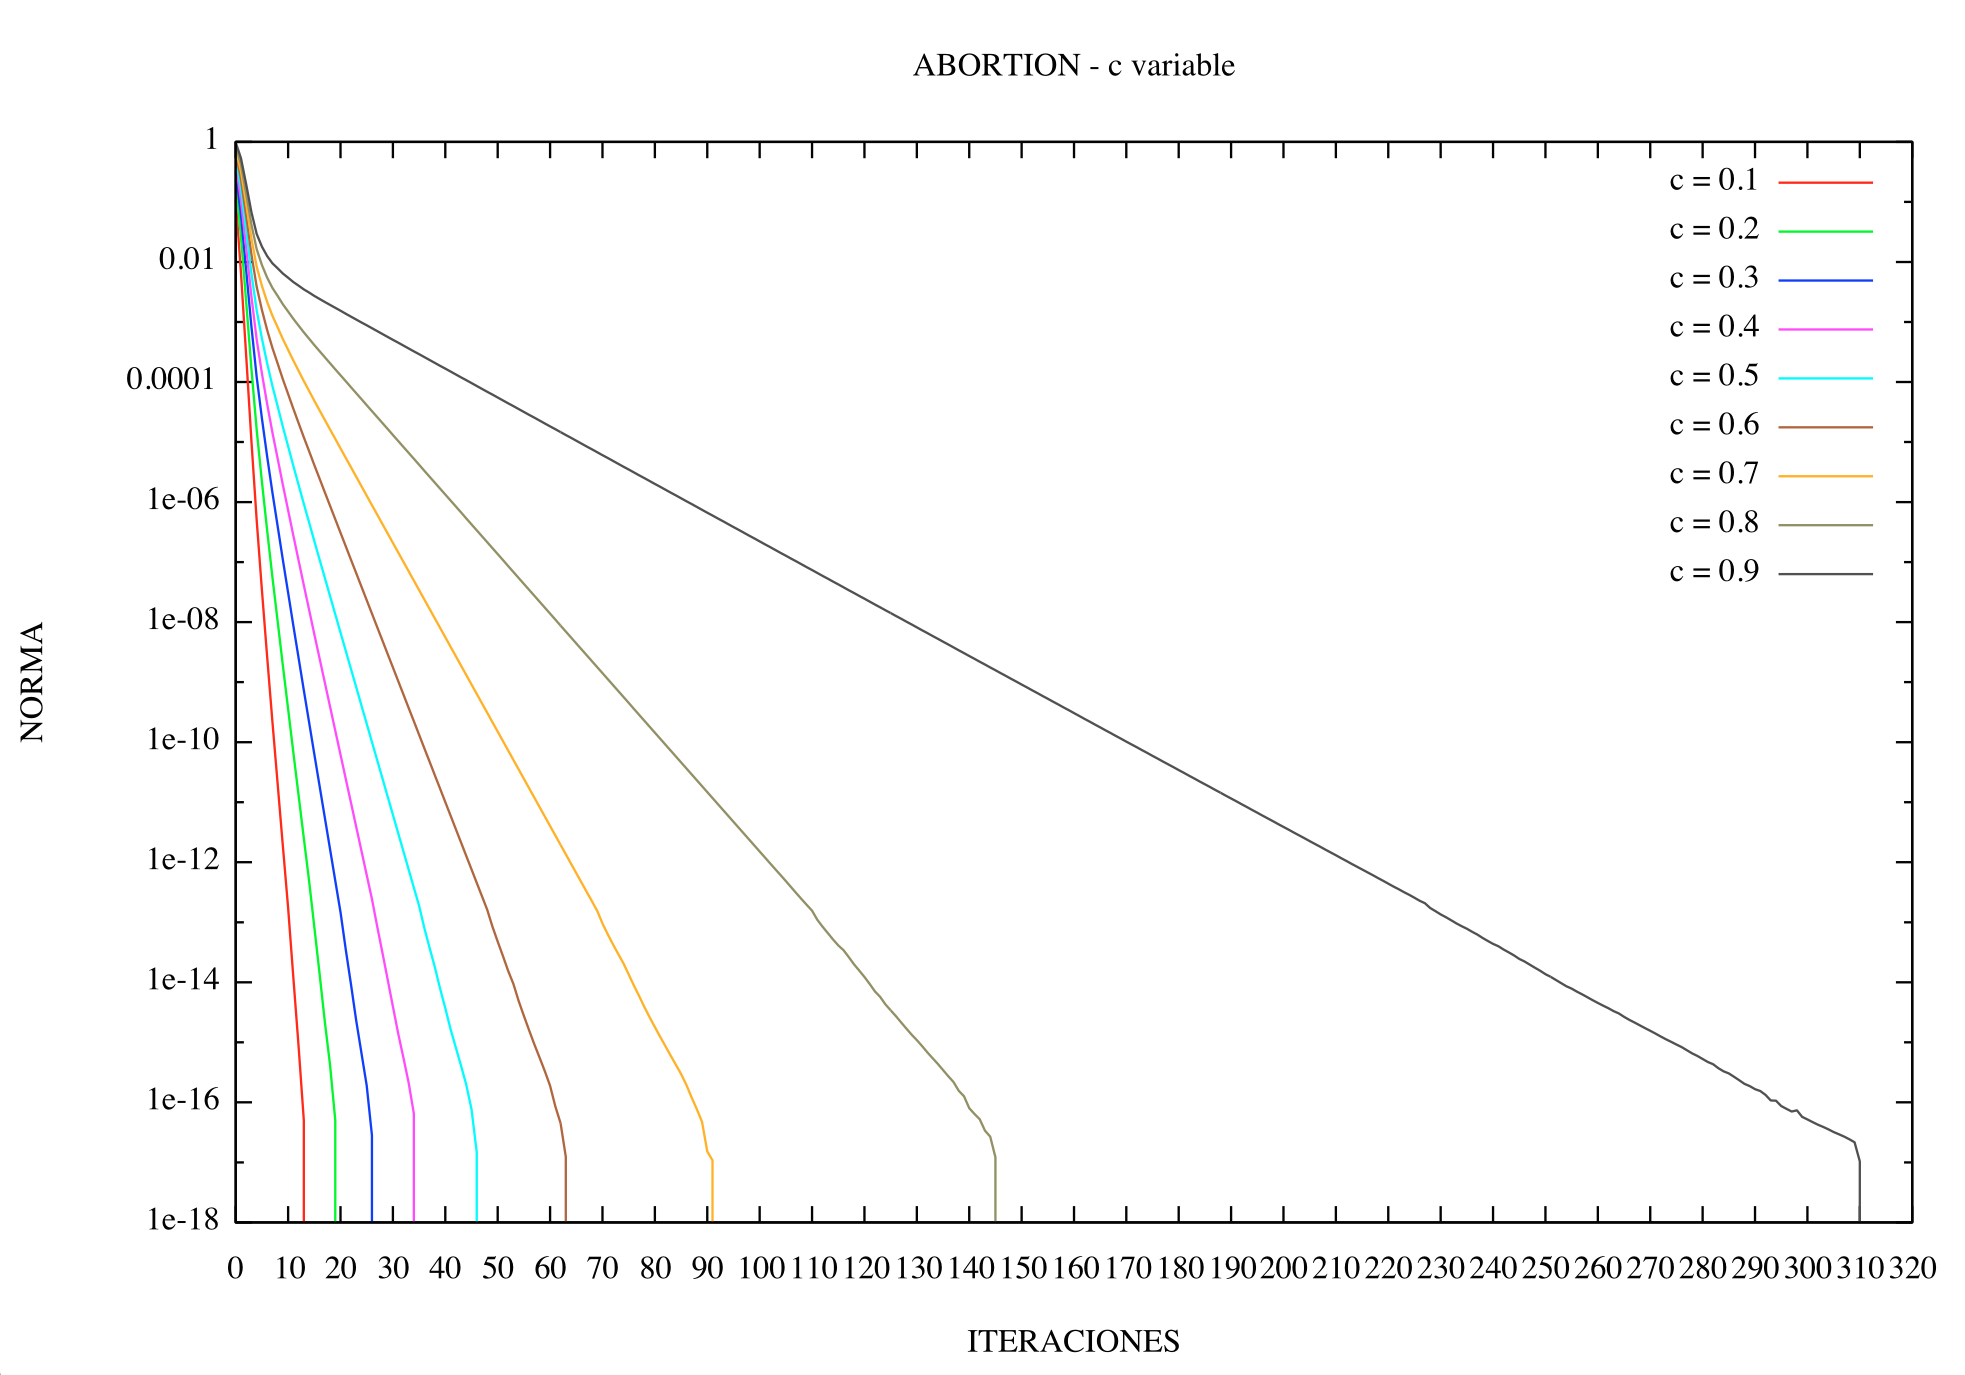
\includegraphics[scale=0.5]{imagenes/pagerank_abortion_norma.png}
       % \end{center}
% \end{figure}

\begin{figure}
\begin{center}
    % 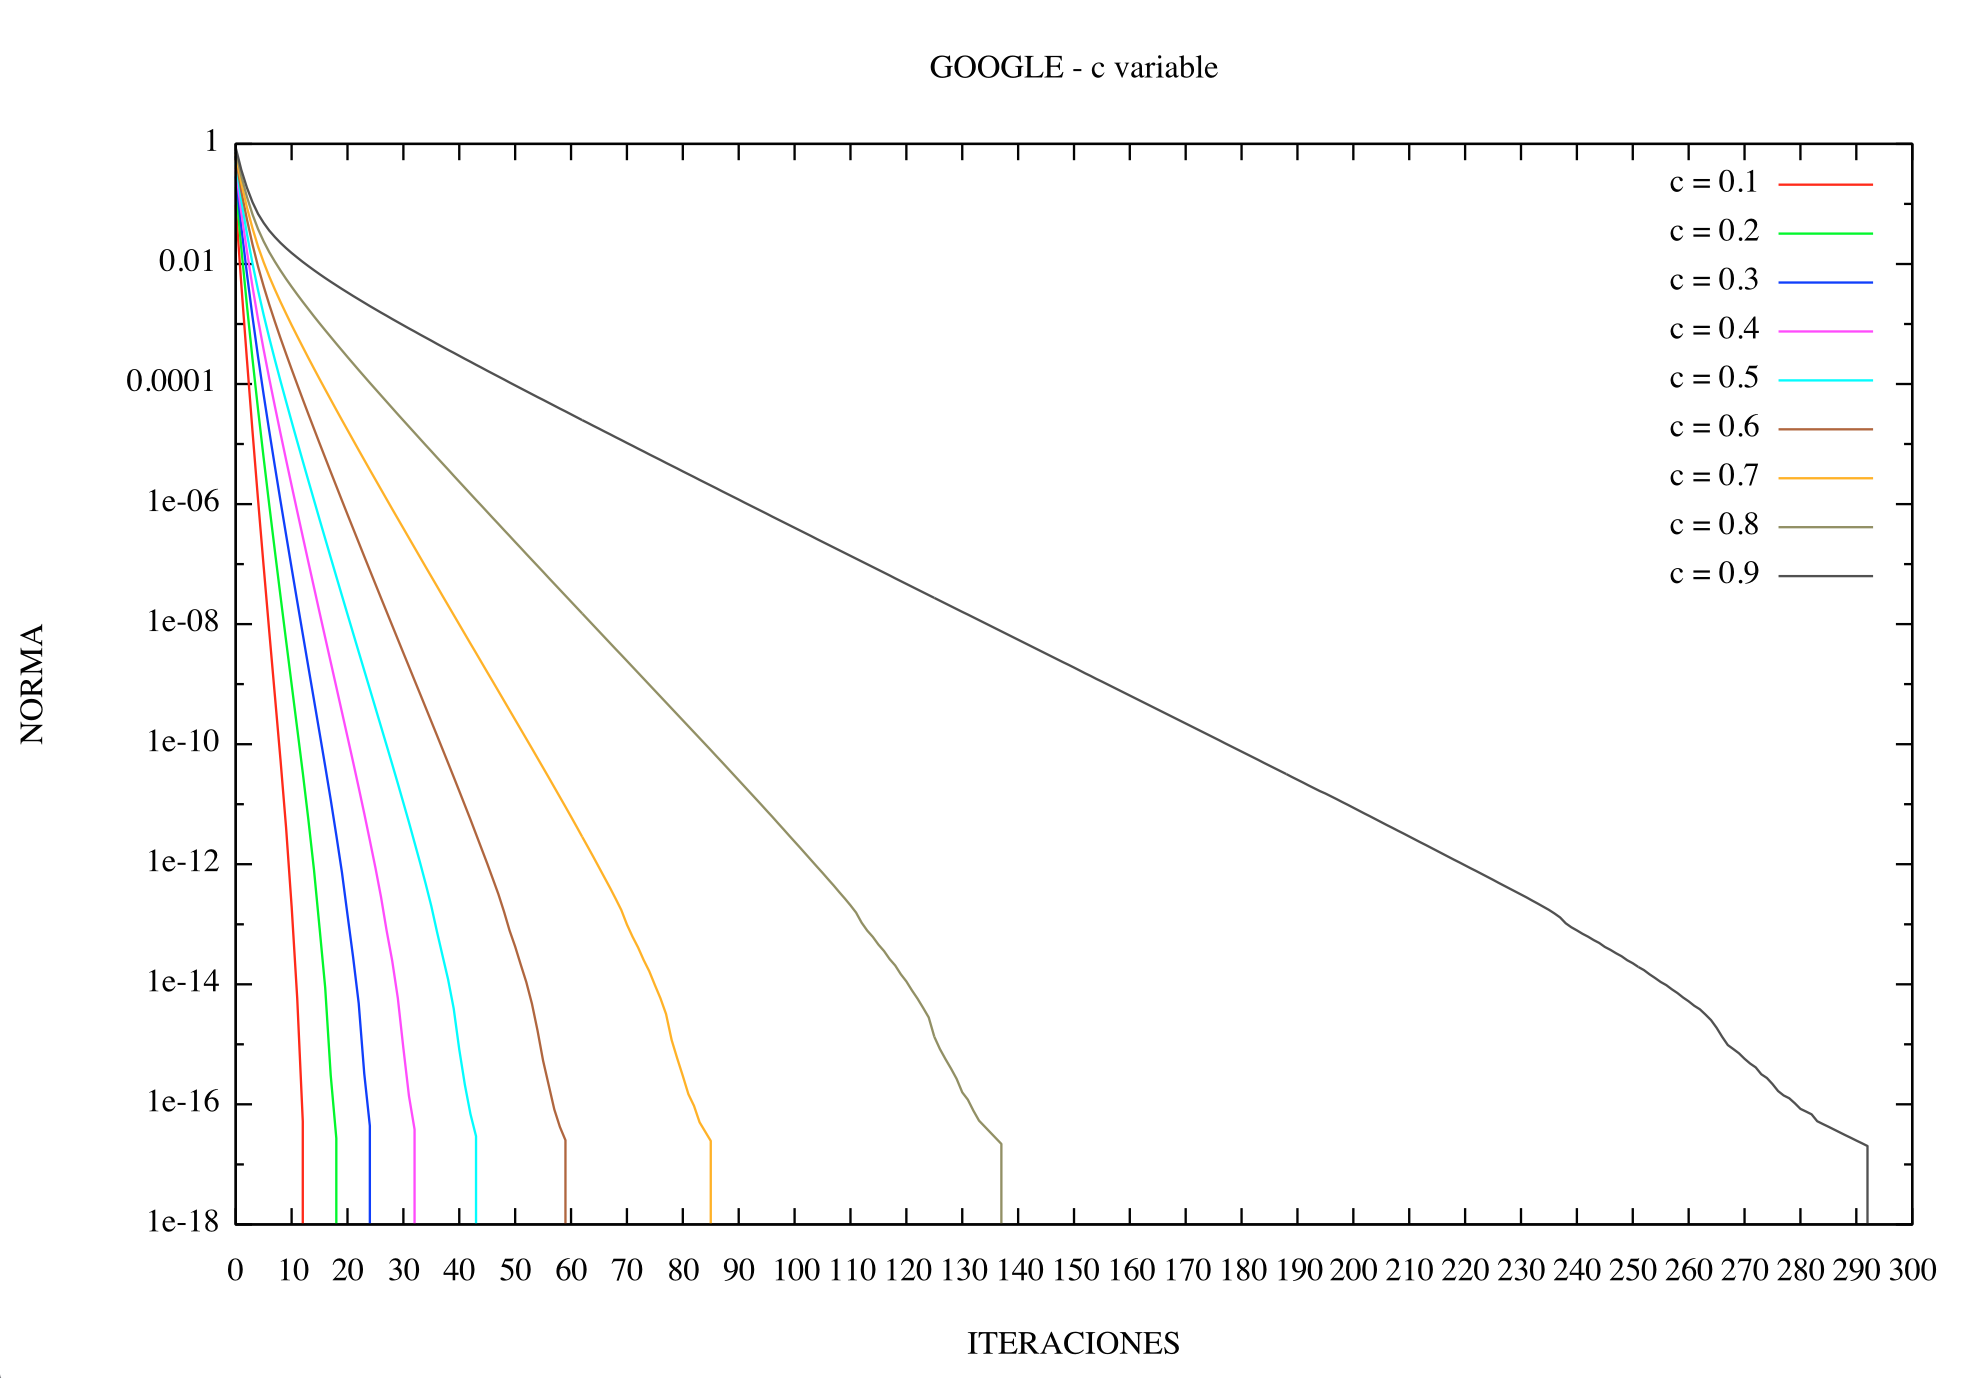
\includegraphics[scale=0.5]{imagenes/pagerank_google_norma.png}
  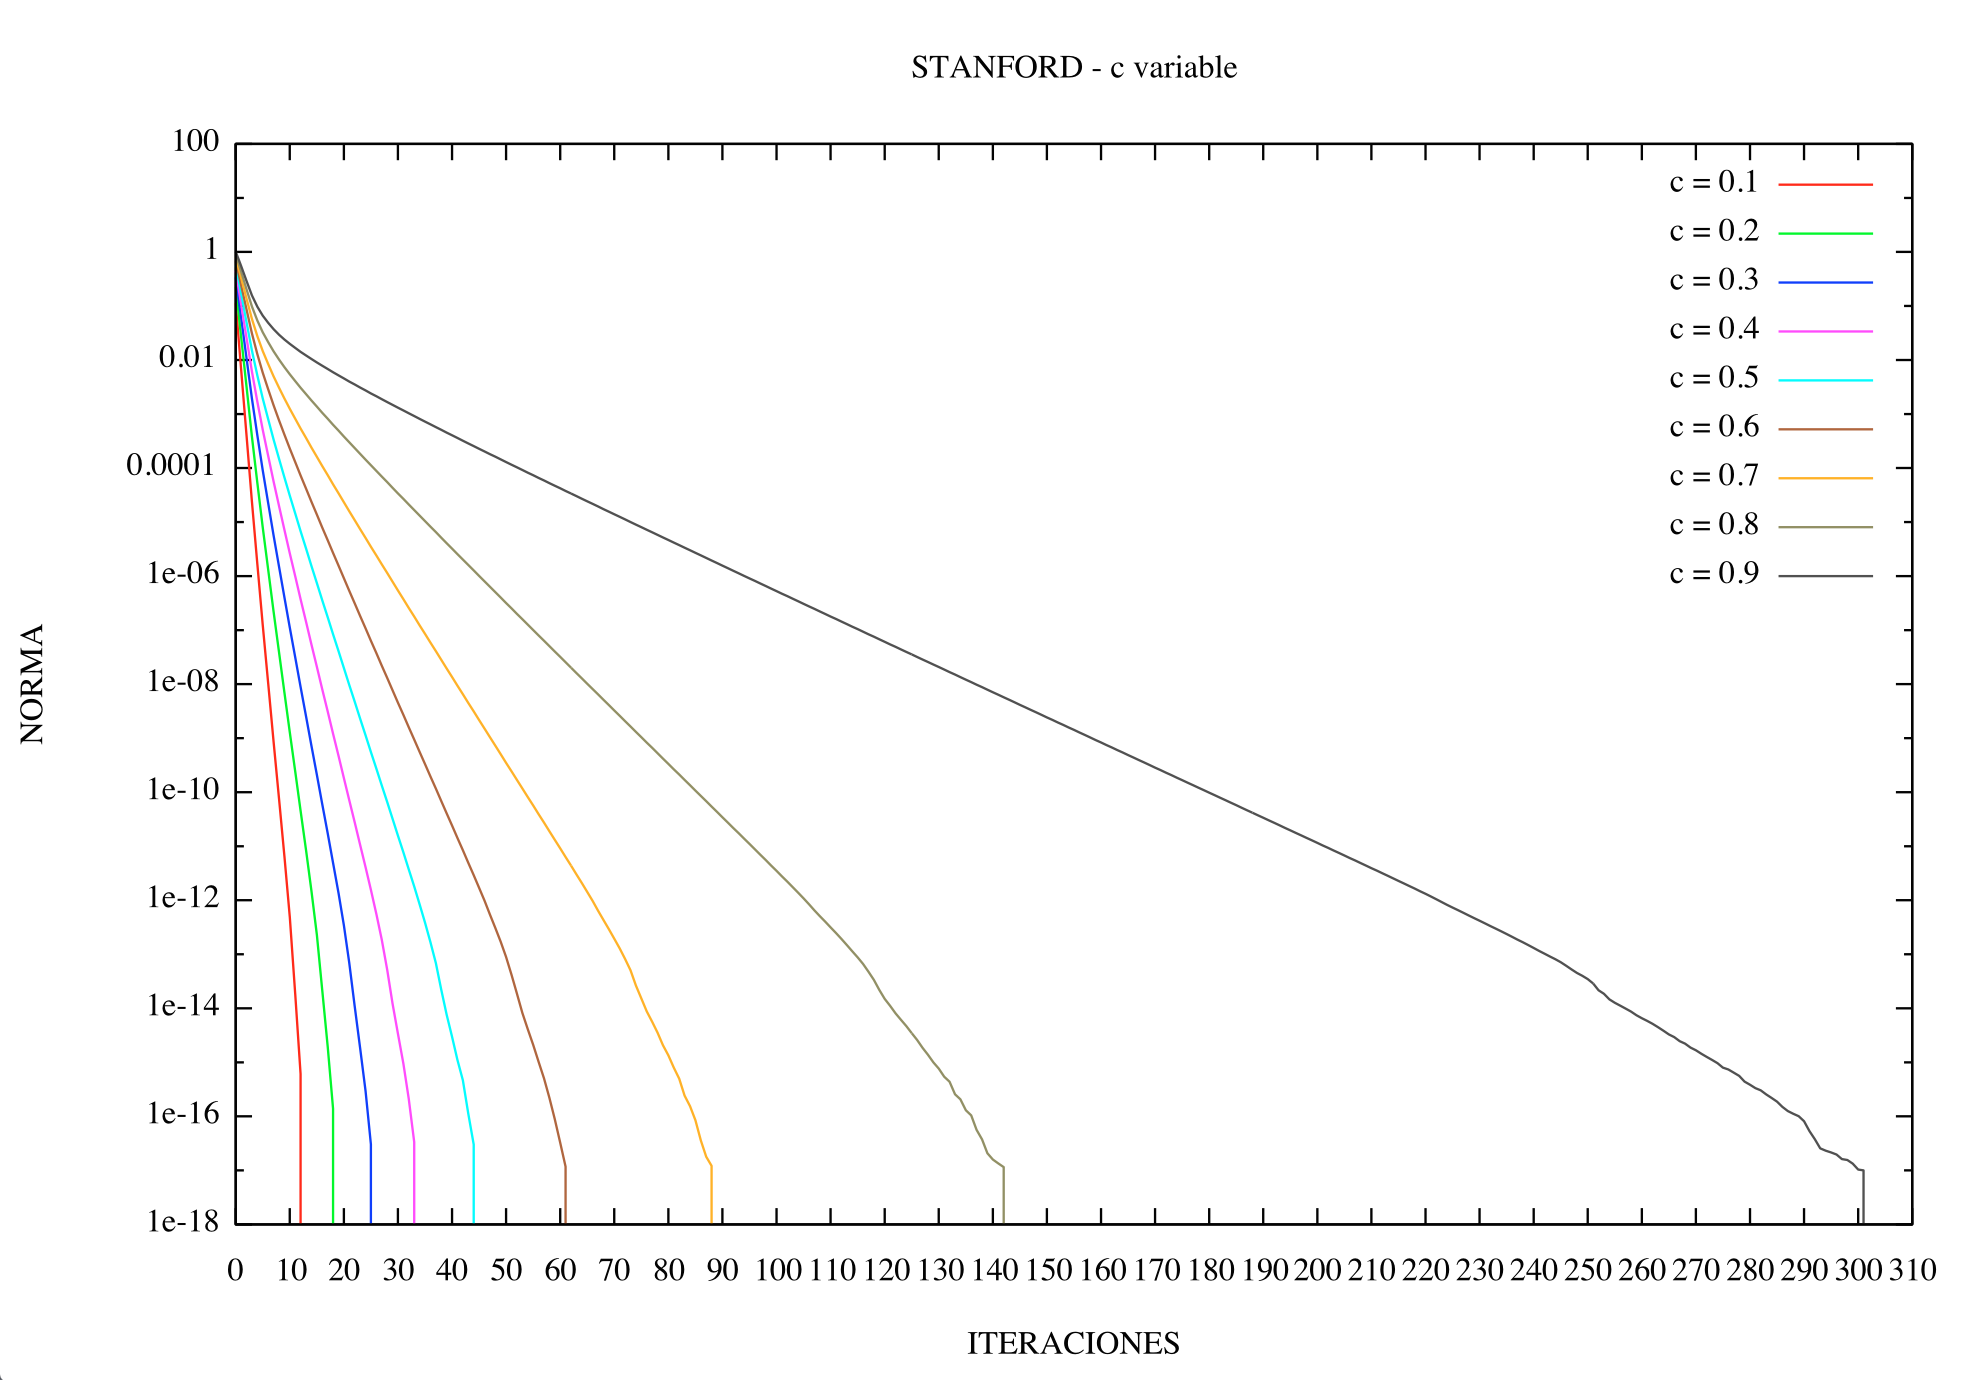
\includegraphics[scale=0.5]{imagenes/pagerank_stanford_norma.png}
    \end{center}
\end{figure}

De los casos de prueba presentados, agregamos solo este ya que el resto de los resultados eran iguales. Claramente notamos que la convergencia se retrasa más a medida que se agranda el c. 

\FloatBarrier

\subsection {Convergencia de HITS}

La convergencia de dicho algoritmo ocurrirá cuando la norma Manhattan de los vectores x e y (que contienen el puntaje de los sitios de autoridad y los de hubs respectivamente) comparados con los de la iteración anterior sea cero para alguno de los dos(o a un valor relativamente cerca). Es ahí cuando tendremos la respuesta final.\\
Al igual que el algoritmo anterior utilizamos una tolerancia igual a cero.

A continuación se muestran los resultados para cuatro instancias distintas, una medianas y una grande, de como evoluciona la norma a lo largo de las iteraciones en ambos vectores :
\begin{figure}[!htb]
\begin{center}
       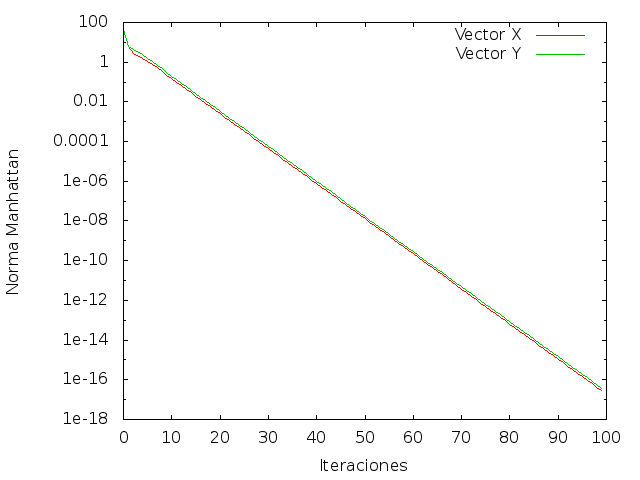
\includegraphics[scale=0.5]{imagenes/hits-abortion-expanded.png}
       \caption{Abortion expanded }
  \end{center}
\end{figure}
\begin{figure}[!htb]
\begin{center}
        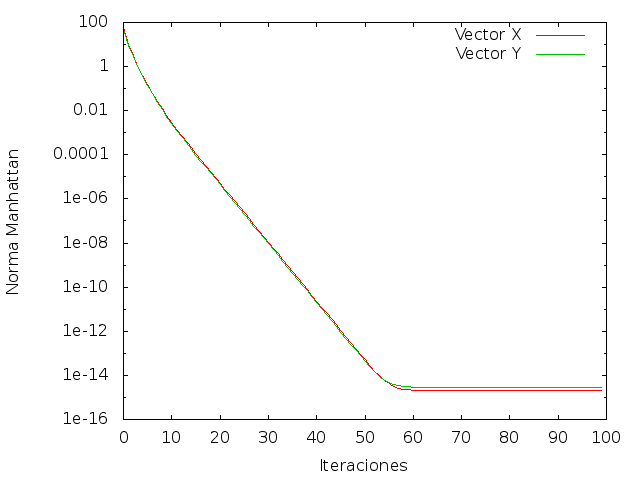
\includegraphics[scale=0.5]{imagenes/hits-genetic-expanded.png}
       \caption{Genetic expanded }
       \end{center}
\end{figure}

\begin{figure}[!htb]
\begin{center}
    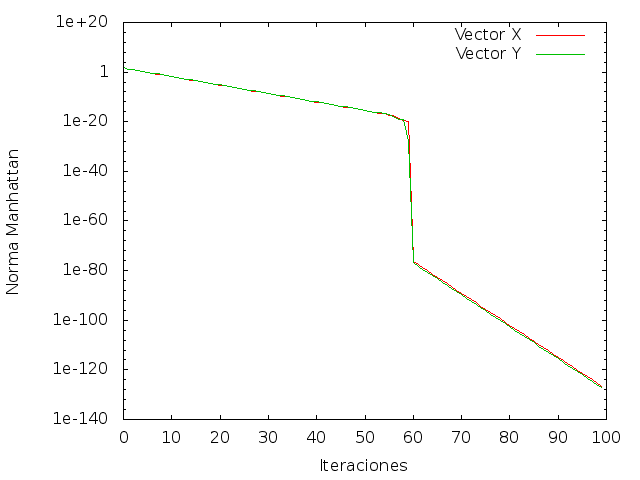
\includegraphics[scale=0.5]{imagenes/hits-movie.png}
    \caption{Movies expanded }
  \end{center}
\end{figure}
\begin{figure}[!htb]
\begin{center}
    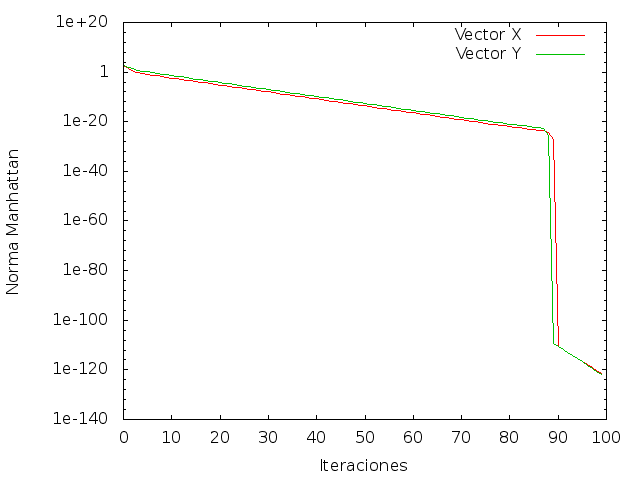
\includegraphics[scale=0.5]{imagenes/hits-stadfor.png}
    \caption{Standford}
    \end{center}
\end{figure}

\subsection{Comparación de Tiempos}

El siguiente gráfico muestra la evolución del tiempo de computo en función del tamaño de la red para cada algoritmo. La red utilizada en todos los casos es una red estrella en la que todos los nodos (o sitios) apuntan al primero de ellos. Utilizamos este tipo de grafo ya que en c++ es el más rápido y simple de crear teniendo en cuenta además que la forma del grafo no tiene un impacto de eficiencia en los algoritmos sino su tamaño en nodos y aristas es el que cambia el tiempo de ejecución. Por esto no nos pareció pertinente probar distintos tipos de grafos (arboles, completos, bipartito, etc) sin más bien el tamaño de los mismos.

 \begin{figure}[!htb]
\begin{center}
    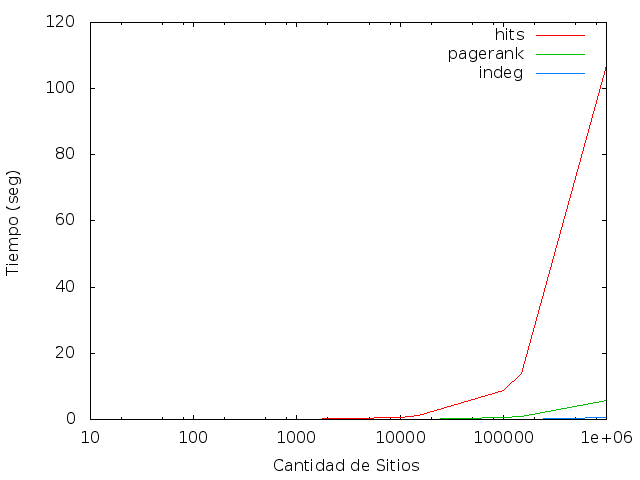
\includegraphics[scale=0.5]{imagenes/Tiempos.png}
    \caption{Tiempo de ejecución en función del tamaño de la red}
    \end{center}
\end{figure}



